\chapter{Literature Review}
\label{sec:Literature Review}

A literature review has been conducted for this project. This section of the report documents the relevant research performed and divides into to the following sections:
\begin{itemize}
    \item \textbf{\hyperref[sec:Laparoscopy Overview]{Laparoscopy Overview}:} An overview of what laparoscopy is and its history.
    \item \textbf{\hyperref[sec:Current Technological Advancements]{Current Technological Advancements}:} The current directions that modern laparoscopy is improving on.
    \item \textbf{\hyperref[sec:Current Available Technology]{Current Available Technology}:} A summary of current Laparoscopes that is available in South Africa.
    \item \textbf{\hyperref[sec:Available Hardware Components]{Available Hardware Components}:} An overview of different hardware modules available for this project.
    \item \textbf{\hyperref[sec:Software Considerations]{Software Considerations}:} An brief overview of the available programs that can be used for this project.
    \item \textbf{\hyperref[sec:Visual Inspection Considerations]{Visual Inspection Considerations}:} An overview of visual inspection and aspects of camera that need to be mastered.
\end{itemize}

\section{Laparoscopy Overview}
\label{sec:Laparoscopy Overview}

Laparoscopy is a branch of the endoscopic medical field. It has become an integral part of surgical procedures in all field in the recent decades. Inspired by the minimally invasive surgery (MIS) approach, laparoscopic surgery consist of making 1 or more small incisions on the abdomen of the patient. Surgeons use these incision to insert thin rod medical equipment into the patient to perform the surgery. \citep{FIS-2021}

\vspace{0.5cm}
\noindent An essential tool of this surgical procedure is the laparoscope. Due to small size of the incisions, the surgeons' view is limited. The laparoscope is the solution to this problem. It allows the surgeons to view what is occurring within the patient while the operation is being performed. Therefore, they can clearly manipulate their equipment from outside the patient to perform complex procedures inside the patient. \citep{AIP-2018}

\vspace{0.5cm}
\noindent There are 2 design methods being used currently when developing laparoscopes. Their main difference is the placement of the digital camera on the tool itself. The first method is inspired by the \textit{\hyperref[fig:old laparoscope]{original laparoscope design}}. This method utilized reflective lenses and cold light sources, which allowed the surgeon to inspect the abdomen of a patient, similar fashion as a microscope. However, instead of an eye piece, a camera is used so that the captured digital images can be displayed in real-time to the surgical staff.\citep{FIS-2021}

\begin{figure}[htbp]
    \centering
    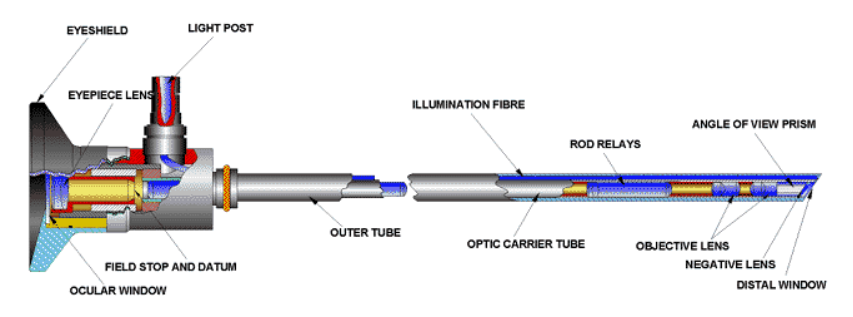
\includegraphics[height = 5cm]{figs/Endoscope.png}
    \caption{Original laparoscope design. \citep{EBME-2026}}
    \label{fig:old laparoscope}
\end{figure}

\noindent The second design method use to develop laparoscope utilizes chip on stick technology. \citep{WLH-M} This design method places the camera of the laparoscope on the tip of the tool. This method removes the complex lenses required for the traditional and use a variety of wide lens camera modules. \citep{AIP-2018}

\noindent Laparoscopic surgery has been one of the greatest advancements in medical industry in recent years. \textit{\citet{WJM-2015}} shows that laparoscopic surgery has quicker recovery time and less pain after surgery compared to traditional open surgery. However, it shows that certain procedures are more time-consuming and more complex to perform.


\section{Current Technological Advancements}
\label{sec:Current Technological Advancements}

Since the addition of cameras to laparoscopes, there has been a large addition of advancement available. These advancement range from hardware improvements to additional software programming abilities to the existing design.

\vspace{0.5cm}
\noindent The main hardware advancement made to the camera module is increasing the field of view (FoV). However, there are additional advancements made in hardware for laparoscopes. The addition of robotics to the laparoscopes has greatly assisted the laparoscopic surgical industry. Robotic manipulators are utilized to assist surgeons by maintaining stable control of the laparoscope, therefore, ensuring consistent and clear visualization during the procedure.\citep{AIP-2018}

\vspace{0.5cm}
\noindent There are multiple additions currently being made to the software of laparoscopes. \textit{\citet{AIP-2018}} list the following additions: 

\begin{itemize}
    \item Digital imaging enhancement techniques.
    \item AI incorporation.
    \item 3D visualization.
    \item Object tracking.
\end{itemize}

\section{Current Available Technology}
\label{sec:Current Available Technology}

There is a range of different laparoscope or endoscope suppliers. Each of these suppliers produce more than 1 product. Therefore, only suppliers for South African hospitals will be reviewed and Intuitive Surgical that produces the \textit{Da Vinci} system, that has been dominating the surgical robot market. \citep{AIP-2018}

\vspace{0.5cm}
\noindent One of the main suppliers of laparoscopic equipment in South Africa is Karl Storz Endoskope, a German company, with a sales office in Cape Town. They produce various products in the medical industry. \citep{KSE-HP} One of their products is the \textit{\hyperref[fig:TIPCAM1]{TIPCAM1 RUBINA}}.

\vspace{0.5cm}
\noindent \textit{\hyperref[fig:TIPCAM1]{TIPCAM1 RUBINA}} is a rigid endoscope with the ability of 0° and 30° viewing angle. It also comes with automatic horizon control and the ability to easily swap between 2D and 3D imaging. Its has an outer diameter of 10.3 mm and a working length of 320 mm. It is has 4K image resolution and has a mass of 420 g. \citep{KSE-TR}
\begin{figure}[htpb]
    \centering
    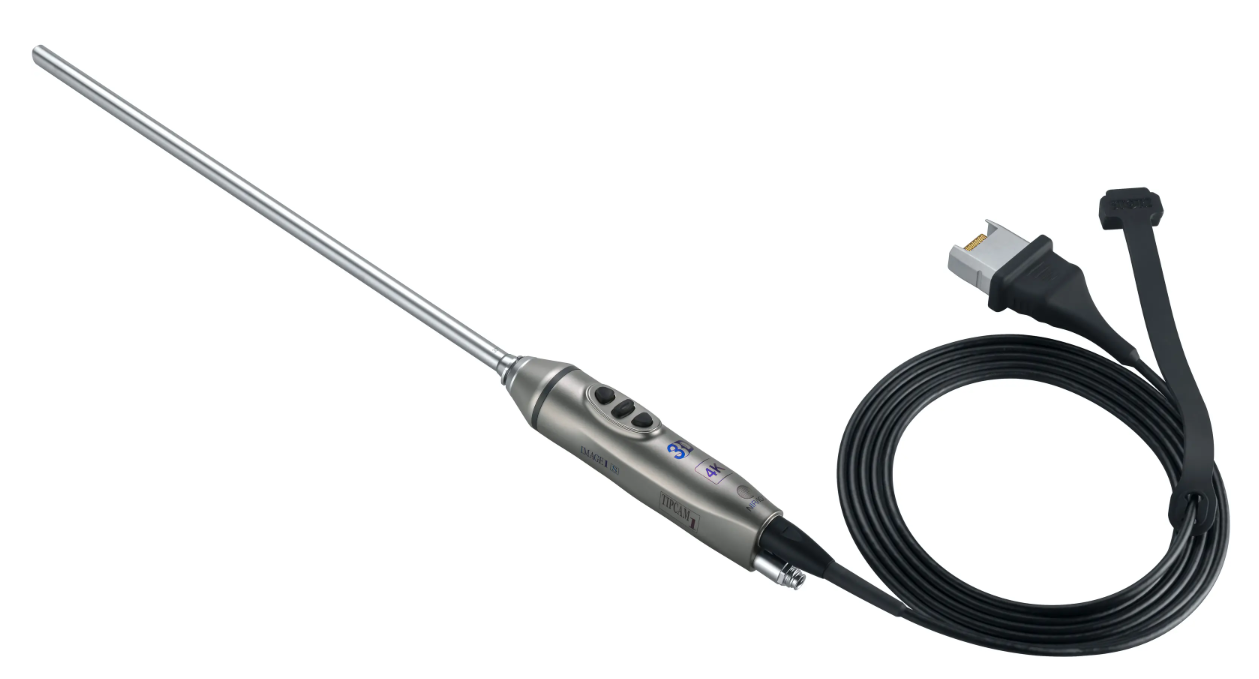
\includegraphics[width=0.5\linewidth]{figs/TIPCAM1 RUBINA.png}
    \caption{Figure of the TIPCAM1 RUBINA. \citep{KSE-TR}}
    \label{fig:TIPCAM1}
\end{figure}

\noindent Olympus Corporation is another company that supplies medical equipment globally. They are a Japanese manufacturing company that produces the \textit{\hyperref[fig:ENDOEYE]{ENDOEYE 3D 10 mm}}. The \textit{\hyperref[fig:ENDOEYE]{ENDOEYE 3D 10 mm}} is a video telescope, with the ability of 3D imaging at a viewing angle of 0° and 30°. It is able to perform image rotation at 30° viewing angle, while maintaining the horizon. \citep{OC-E}

\begin{figure}[htpb]
    \centering
    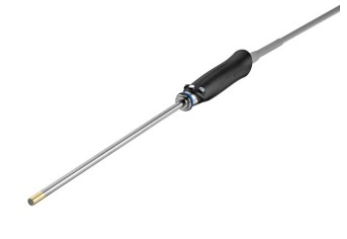
\includegraphics[width=0.5\linewidth]{figs/ENDOEYE 3D 10mm.png}
    \caption{Figure of the ENDOEYE 3D 10 mm. \citep{OC-E}}
    \label{fig:ENDOEYE}
\end{figure}

\noindent Certain international companies uses local distributors to sell their products. Intuitive Surgery, an American company, uses this method. They designed and manufacture the \textit{Da Vinci} medical robot. This system has various variants for different surgical purposes. Currently, there is \textit{Da Vinci Xi} and \textit{Da Vinci X} for multi port surgery. However, the \textit{Da Vinci SP} is designed for single port surgery. These robot systems are are equipped with 7 DOF movement and 3D visualization. Their only drawback is there large size and enormous financial procurement cost. \citep{IS-SP}Below is a figure of the \textit{\hyperref[fig:Da Vinci]{Da Vinci SP}}.

\begin{figure}[htpb]
    \centering
    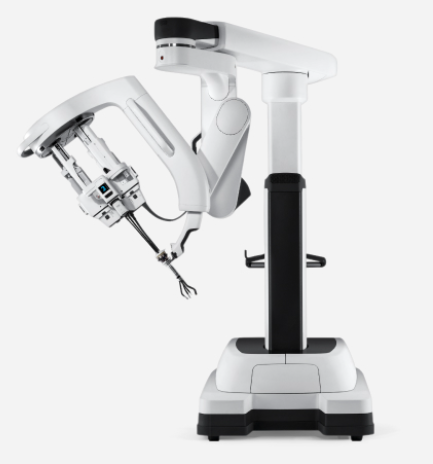
\includegraphics[width=0.5\linewidth]{figs/Da Vinci SP.png}
    \caption{Figure of the Da Vinci SP. \citep{IS-SP}}
    \label{fig:Da Vinci}
\end{figure}

\section{Available Hardware Components}
\label{sec:Available Hardware Components}

There multiple hardware components required to build a laparoscope. Therefore, this section will be divided into multiple subsection where different products will be reviewed for each component. These subsections include: 
\begin{itemize}
    \item \hyperref[sec:Main Microcontroller and Computer Module]{Single board computer module.}
    \item \hyperref[sec:Camera Module]{Camera module.}
\end{itemize}

\subsection{Single Board Computer Module}
\label{sec:Main Microcontroller and Computer Module}

Single board computers (SBC) is a credit-card-size computer, able to perform complex computations while operating various systems. For the laparoscope, it will be the main "brain" of the system. Therefore, it is critical that it can perform all necessary tasks it requires. There is 2 main suppliers of SBC:
\begin{itemize}
    \item Raspberry Pi Ltd.
    \item Arduino AG.
\end{itemize}

\noindent Raspberry Pi has a large range of products that is available for the project. However, Raspberry Pi's SBCs has an important feature installed into most of SBC, that would be beneficial to the project. This feature is the designated camera serial interface (CSI) or the MIPI camera display transceivers, according to Raspberry Pi. This feature allows for high-quality videos at high speeds. \citep{RP-DOC} The \textit{\hyperref[tab:Raspberry Pi SBC]{table}} below show the available options of all the Raspberry Pi SBC:

\begin{table}[H]
    \centering
    \caption{Raspberry Pi SBCs.\citep{RP-P}}
    \begin{tabular}{|c|c|c|c|c|}
    \hline
        Raspberry Pi SBC & RAM & CPU Speed & MIPI Ports & Cost \\
    \hline
        Pi 5 & 1-16 GB & 2.4 GHz & 2 & R 3 266.00\\
    \hline
        Pi 4 Model B & 1-8 GB & 1.5 GHz & 1 & R 1 360.00\\
    \hline
        Pi 3 Model B+ & 1 GB & 1.4 GHz & 1 & R 640.43\\
    \hline
        Pi Zero 2 W & 512 MB & 1 GHz & 2 & R 240.16 \\ 
    \hline
        Pi Zero 2 & 512 MB & 1 GHz & 2 & R 309.90 \\ 
    \hline
    \end{tabular}
    \label{tab:Raspberry Pi SBC}
\end{table}

\noindent All of the SBC in \textit{\hyperref[tab:Raspberry Pi SBC]{table}} above have these features:

\begin{itemize}
    \item 40 GPIO Pins.
    \item Wi-Fi Capabilities.
    \item Bluetooth Capabilities.
\end{itemize}

\noindent Arduino, similar to Raspberry Pi, have a wide range of products available for this project. However, they have one absent feature, namely the lack of CSI feature. Therefore, they are incompatible with the Raspberry Pi Camera Modules. However, they can use other camera modules, with the use of SPI and I2C GPIO pins. Although this options isn't favourable, due to trade-off in quality during longer videos, it is still a feasible option that can be explored. \citep{GH-AA} The \textit{\hyperref[tab:Arduino SBCs]{table}} below shows the available products from Arduino:

\begin{table}[H]
    \centering
    \caption{Arduino SBCs. \citep{A-P}}
    \begin{tabular}{|c|c|c|c|c|}
        \hline
            Arduino SBC & RAM & CPU Speed & SPI Ports & Cost \\
        \hline
            UNO R4 WiFi & 32 kB & 48 MHz & 1 & R 488.46 \\
        \hline 
            UNO R4 Minima & 32 kB & 48 MHz & 1 & R 352.33 \\
        \hline
            UNO R3 & 2 kB & 16 MHz & 1 & R 469.24\\
 %       \hline
%            Mega 2560 Rev 3 & 8 kP & 
        \hline
            GIGA R1 WiFi & 1 MB & 480 MHz & 2 & R 1 247.58 \\
        \hline
            Nano ESP32 & 512 kB & 240 MHz & 1 & R 358.74 \\
        \hline
            Nano RP2040 Connect & 264 kB & 133 MHz & 4 & R 389.17 \\
        \hline
            UNO Q & 2 GB & 2 GHz & 1 & R 1 035.54 \\
        \hline
            Nano 33 BLE & 256 kB & 64 MHz & 4 & R 456.43 \\
        \hline
            Nano 33 IoT & 520 kB & 240 MHz & 6 & R 427.6 \\
        \hline
            Nano Every & 6 kB & 20 MHz & 1 & R 232.22 \\            
        \hline
    \end{tabular}
    \label{tab:Arduino SBCs}
\end{table}

\subsection{Camera Module}
\label{sec:Camera Module}

The camera module is another important component of this project. It is essential to capture the real-time images inside the patient. Therefore, this component should be selected carefully. A common occurrence with the camera modules is that the size of the camera sensor and assembly can fit in a Ø10 mm hole. However, the circuit board that it is attached to it does not fit inside this hole. Therefore, options with removable camera assemblies that can be attached to the circuit board with a wire connection were reviewed. Consequently, camera modules that already fit inside with the hole, that comes with a wire extension is reviewed as well. 

\vspace{0.5cm}
\noindent Raspberry Pi camera modules all have all circuit board connection, that can't separate from the camera sensor, as can be seen in the \textit{\hyperref[fig:Raspberry Pi Camera Module 3]{figure}} below. However, it is optional to purchase the stand-alone sensor assembly for the Raspberry Pi camera module V3. Although, this camera sensors it powerful, with IMX708 sensor capable of 4608 x 2592 pixels images, it physical size is 10.8 mm x 10.8 mm. Therefore, it is incapable to fit inside the Ø10 mm hole. \citep{AC-RP}


\begin{figure}[htpb]
    \centering
    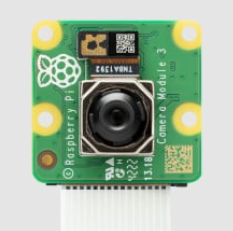
\includegraphics[width=0.5\linewidth]{figs/Raspberry Pi Camera Module V3.png}
    \caption{Figure of Raspberry Pi Camera Module 3}
    \label{fig:Raspberry Pi Camera Module 3}
\end{figure}

\vspace{0.5cm}
\noindent As mention in the previous section, \textit{\hyperref[sec:Main Microcontroller and Computer Module]{Single board computer module}}, the Raspberry Pi SBC modules have CSI ports. Even though Raspberry Pi camera modules can't be considered for this project, other suppliers make camera modules that can interface with these CSI ports. Below is a \textit{\hyperref[tab:Leopard Imaging camera modules]{table}} of the supplier, Leopard Imaging, from their hummingbird mobile camera modules series:

\begin{table}[H]
    \centering
    \caption{Leopard Imaging camera modules.\citep{LI-P}}
    \begin{tabular}{|c|c|c|c|c|}
    \hline
        Product code & Resolution & Max fps & FoV (°) & Focus depth \\
    \hline
         LI-OV2685-MIPI-FF & 2 MP & 120 & 60 & 30 cm - inf  \\
    \hline 
        LI-OV8865-MIPI-AF & 8 MP & 60 & 70 & 10 cm - inf  \\
    \hline
        LI-OV13850-MIPI-AF & 13 MP & 30 & 70 & 10 cm - inf  \\
    \hline
        LI-OV5640-MIPI-AF & 5 MP & 120 & 65 & 10 cm - inf  \\
    \hline
        LI-AR1335C-MIPI-061H-AF & 13 MP & 30 & 61 & 10 cm - inf  \\
    \hline
        LI-IMX258-MIPI-AF & 13 MP & 60 & 79.8 & 10 cm - inf  \\
    \hline
        LI-IMX586-MIPI-AF-79D & 48 MP & 240 & 79 & N/A \\
    \hline
        LI-IMX681-MIPI-AF-96D & 12 MP & 30 & 96 & N/A  \\
    \hline
        LI-AR0246-FLEX-80H & 2 MP & 60 & 80 & 35 cm - inf  \\
    \hline 
        LI-OV16E10-AF-D78 & 16 MP & 120 & 78.4 & 7 cm - inf \\
    \hline
        LI-AR0544-MIPI-150H & 5 MP & 60 & 150 & 15 cm - inf \\
    \hline
        LI-OS04C10-MIPI-107H & 4 MP & 240 & 107 & 70 cm - inf\\
    \hline
        LI-OG12B10-MIPI-AF-95D & 12 MP & 240 & 75 & 10 cm - inf \\
    \hline
        LI-OV13B10-MIPI-AF-75D & 13 MP & 60 & 75 & 10 cm - inf \\
    \hline
        
    \end{tabular}
    
    \label{tab:Leopard Imaging camera modules}
\end{table}

\noindent Another camera module manufacturer is ArduCam Technology Co., Ltd. They specialize in embedded camera modules and is a leading company in the designing of camera modules. They also produce several camera modules, however, their most relevant product to this project is their \textit{\hyperref[fig:Arducam Spy Camera]{OV5647 Spy Camera module}}. Here is a list of the products specifications:

\begin{itemize}
    \item Resolution: 5 MP.
    \item Max fps: 90.
    \item FoV: 120°.
    \item Cost: R 316.89    
\end{itemize}

\noindent This product however does have one flaw. Its focus depth is 1 m to inf.\citep{A-P} Therefore, this product cannot be used for this project.

\begin{figure}[htpb]
    \centering
    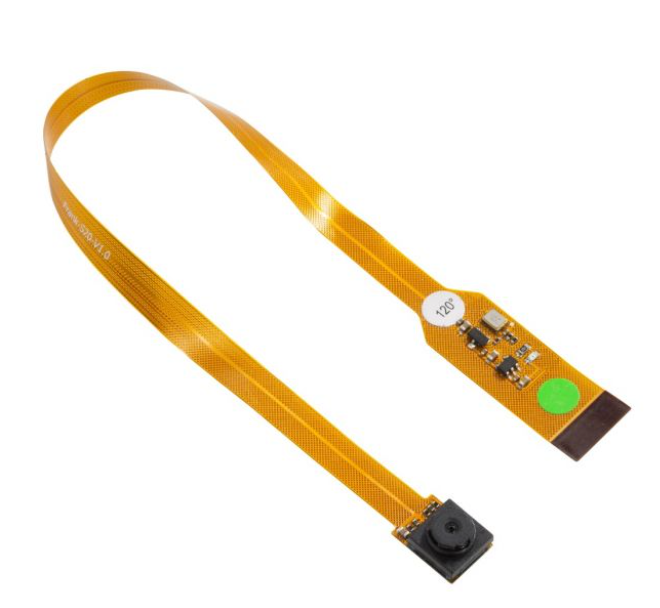
\includegraphics[height = 4cm]{figs/Arducam Spy camera.png}
    \caption{Figure of Arducam spy camera module.\citep{A-P}}
    \label{fig:Arducam Spy Camera}
\end{figure}


\noindent For this project, there is an option of purchasing endoscope camera modules. These camera modules are designed to be used in a endoscopic application. There are various designers and manufacturers and each of these have their own series of products.

\vspace{0.5cm}
\noindent IADIY Technology is a Chinese company, that creates a line of products that can communicate with USB cable attached to the camera module. Below is a \textit{\hyperref[fig:IADIY camera module]{figure}} of a IADIY camera module. These camera modules are powerful, with their compact size, wide Field-of-View angles and built in light sources. Here is a \textit{\hyperref[tab:IADAY Camera Modules]{table}} that list all the available products from IADIY technology

\begin{figure}[htpb]
    \centering
    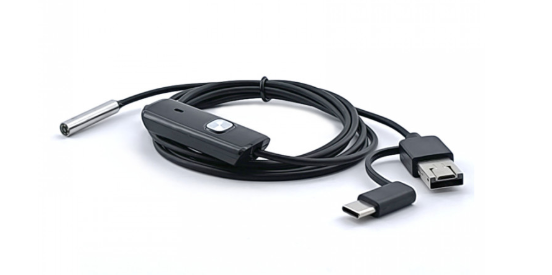
\includegraphics[width=0.5\linewidth]{figs/IADIY camera module.png}
    \caption{Figure of IADIY camera module.\citep{I-E}}
    \label{fig:IADIY camera module}
\end{figure}

\begin{table}[H]
    \centering
    \caption{IADIY endoscopic camera modules. \citep{I-E}}
    \begin{tabular}{|c|c|c|c|c|}
    \hline
        Product Code & Resolution & Ø of Module (mm) & FoV (°) & Max fps  \\
    \hline
        SCM03M30D5.5U & 0.3 MP & 5.5 & 60 & 30  \\
    \hline
        SCM1M30D5.5U & 1 MP & 5.5 & 88 & 30  \\
    \hline
        SCM1M30D3.9U & 1 MP & 3.9 & 140 & 30  \\
    \hline
        SCM2M30D8U & 2 MP & 8 & 80 & 30  \\
    \hline
    \end{tabular}
    \label{tab:IADAY Camera Modules}
\end{table}


\noindent Guangzhou Sincere Information Technology Ltd. (SincereFirst is their trade name) is another Chinese company. They specialize in various camera products that can be used through USB connection. \citep{SF-AU} Below is a \textit{\hyperref[tab:SincereFirst camera modules]{table}} of all the available products from SincereFirst.

\begin{table}[H]
    \centering
    \caption{SincereFirst endoscopic camera modules\citep{SF-CM}}
    \begin{tabular}{|c|c|c|c|c|}
        \hline
            Image sensor & Resolution & Ø of Module (mm) & FoV (°) & Max fps \\
        \hline
            OmniVision OCHFA20 & 720 P & 1.05 & 120 & 30 \\
        \hline
            OmniVision OCHFA10 & 0.5 MP & 1.5 & 105 & 30 \\
        \hline
            N/A & 0.5 MP & 2 & 120 & 30 \\
        \hline
            Brigates ES101 & 1 MP & 3.1 & 140 & 75 \\
        \hline
    \end{tabular}
    \label{tab:SincereFirst camera modules}
\end{table}


\noindent Motoshot Technology Co., Ltd. (Camemake is their trading name) is a Chinese company. Since their establishment in 2016, they have been designing and manufacturing camera modules that can interface with USB, DVP/SPI and CSI. They have 3 endoscopic products that can be considered for this project, as well as a range of other camera module.\citep{CM-HP} Below is a \textit{\hyperref[tab:Camemake camera modules]{table}} that shows some of the products specifications:

\begin{table}[H]
    \centering
    \caption{Camemake endoscopic camera modules. \citep{CM-ECM}}
    \begin{tabular}{|c|c|c|c|c|c|}
    \hline
        Sensor & Resolution & Ø of Module (mm) & FoV (°) & Max fps & Focus Depth\\
    \hline
        N/A & 1080 P & 7 & 60 & 30 & 30 - 50 mm \\
    \hline
        OV2640 & 2 MP & 1.6 & 120 & 30 & 5 - 50 mm \\
    \hline
        OV9734 & 720 P & 4.2 & 100 & 30 & 5 -100 mm \\
    \hline
        
    \end{tabular}
    \label{tab:Camemake camera modules}
\end{table}


\noindent All of these products mentioned above in endoscopic camera module tables, all have built in illumination modules. Thus, minimizing the amount of work required to design and manufacture the developed laparoscope.


\section{Software Considerations}
\label{sec:Software Considerations}

This project is mainly a design problem that has to be addressed. There are however software application needed for this project. The most important application is that of the camera module interface. 

\vspace{0.5cm}
\noindent The software should enable the SBC to connect and operate the camera module. \citet{RP-DOC} properly documents how to use a camera module that interfaces with an CSI connection. If a SPI/I2C connection is required to interface with the camera module, \citet{GH-AA} is library that describes how it can be performed. If  a USB connection is used as an interface between the SBC and camera module, then minimal action is required to interface the 2 modules. \citep{ML-USB} 

\vspace{0.5cm}
\noindent There are however other applications required for this project. As mentioned in the software component of the scope, there are 2 other section of code that need to be considered for this project. The ability display the captured footage to a real-time monitor, depends on the monitor that will be used for this project. If a personal computer is used, the captured footage can be transferred with the means of WiFi, Bluetooth, USB connection, or even a Mathworks ThingSpeak channel.\citep{MW-TS}

\vspace{0.5cm}
\noindent Another important aspect to considered is coding language used for this project. However, this is dependent of the SBC used. If a Raspberry Pi is used, then Python is recommended language to use. \citep{RP-DOC} However, if Arduino is used then the ideal language to use is either C or C++. \citep{A-DOC} Visual Studio Code (VS Code) can be used to perform all programming for this project.

\vspace{0.5cm}
\noindent Documentation of this project will be performed using LaTeX. VS Code will be used to run this application, through the LaTeX Workshop extension.\citep{VS-LW}

\section{Visual Inspection Considerations}
\label{sec:Visual Inspection Considerations}

This project requires a visual camera to be a functional laparoscope. However, there is various factors to be considered to take high-quality images. This section of the literature reviews aims to explain each of these factors. Consequently, how they can impact this project.

\vspace{0.5cm}
\noindent Important concept to understand, is how a digital image is captured. A camera sensors consists of a matrix of millions of light cavities. When a picture is being taken, these cavities, called "photosites", are exposed to the photons of the object or scene. The photons are then collected by the photosites and stored as an electrical charge. Consequently, when the image is finished being taken, these charges are quantified and then processed to make the image. \citep{CC-DCS}

\vspace{0.5cm}
\noindent One aspect that needs to be mastered to captured quality images is the exposure triangle. It is 3 pillars that dictates the quality of an image. Aperture determines the size of the area opened in the lens which light can filter through to sensor. The larger the aperture value, measured in f-stop values, the smaller the hole size where light filters through the lens. This pillars relates to the depth of field of the images. The smaller aperture correlates to shallower depth of field images. \citep{CC-CE}

\vspace{0.5cm}
\noindent Shutter speed is the second pillar to the exposure triangle. When a digital images is being taken the lens opens up to expose the photosites to the light. Consequently, shutter speed refers to total duration of the lens being open, thus causing the sensor to be exposed to image. If the shutter speed increases, then the sensors is exposed to reduced light from the images. Therefore, as the shutter speed increases, the images will gain more quality, with more definitive objects that is more "frozen" in the image. \citep{CC-CE}

\vspace{0.5cm}
\noindent The third pillar is ISO. This determines how sensitive the sensor is to the exposed light. As the ISO value increases, the higher the sensitivity value will become. Therefore, the image will have increased levels of noise captured if the ISO value is increased. \citep{CC-CE}

\vspace{0.5cm}
\noindent Focal length is a critical feature that has to be considered for this project. Focal length, is the distance between the camera sensor and the camera lens. As this value increases, then the field of view value will decrease. Field of view, measured in degrees, is essentially how much of an images can be seen. If this value increases, then a wider image can be taken. \citep{DM-FOW}






